El desarrollo del filtro de {\ttfamily blur} también lo realizamos en
C y en ASM. Este filtro está caracterizado por el radio $r$ y por el
parámetro de difusión $\sigma$. Vamos a utilizar los siguientes
términos

\begin{description}
\item[Marco:] El recuadro de tamaño $r$ que bordea a la figura, donde
  los píxeles no se afectan.
\item[Centro:] La parte de la figura que no es el marco.
\item[Filtro:] La matriz con la que se convoluciona cada píxel.
\item[Vecinos:] Los píxeles cercanos que afectan el valor de salida de
  un píxel en la imagen procesado. Es decir, todos los elementos que
  están a una distancia (en norma 1) menor a $r$ de un píxel dado.
\end{description}

En este filtro, tenemos que aplicar la siguiente relación que
mencionamos en la introducción:

\begin{equation}
  O[i, j, k] = \sum_{x=-r}^{y=r} I[i+x, j+y, k] K_{\sigma, r} [r-x, r-y]
  \label{eq:blur}
\end{equation}

para todos los píxeles en el \emph{centro}. Así, la implementación en
C es, para cada componente $(R, G, B)$ de cada píxel $(i, j)$ del
\emph{centro}, hacer un ciclo en $(x, y)$ entre $(-r, -r)$ y $(r,r)$.
Un detalle es la identificación del vecino $(x, y)$ del pixel $(i, j)$
con la posición absoluta en la imagen,
$(i + x, j + y) = (i + x)*n_{\text{cols}} + (j + y)$. Así, con los
valores de $(R, G, B)$ del píxel $(i, j)$ de la imagen salida
inicializados a 0, acumulamos en cada uno
$ I[i+x, j+y] K_{\sigma, r} [r-x, r-y]$. Luego, redondeamos este
resultado (que es de punto flotante de 4 bytes) a un char y lo
guardamos en la imagen de salida.

Unas consideraciones hay que realizar en el cálculo del filtro:

\begin{enumerate}
\item Normalización: a pesar de que la función gaussiana está
  normalizada a 1, no sucede en este caso (ya que está discretizada y
  además truncada). De este modo, el coeficiente de normalización del
  filtro tiene que ser calculado para cada uno, de modo tal que la
  suma de todos los elementos de la matriz sea 1.

\item Cálculo: para calcular los elementos de una gaussiana hay que
  realizar muchos cálculos de punto flotante. Para evitarnos repetir
  estos cálculos una y otra vez, y como el filtro es siempre el mismo,
  lo implementamos como una \emph{look up table} y lo guardamos en la
  memoria\footnote{Como esta matriz es utilizada muy seguido, intuimos
    que se mantiene siempre en cache, de forma tal que su acceso sería
    bastante rápido.}. La creación de la LUT es en C [de cualquier
  modo, esta cuenta se realiza \emph{una sola vez por imagen}, así que
  no es costoso su cálculo].
\end{enumerate}

La implementación en ASM fue realizada nuevamente utilizando las
instrucciones {\ttfamily SSE}. Para eso, tenemos que vectorizar el
filtro. Llamando $\mathbf{T}$ a la matriz de píxeles de salida (es decir,
$\mathbf{T}[i, j] = \mathbf{t}_{i, j} = (R^s_{i, j}, G^s_{i, j},
B^s_{i, j})$)
y $\mathbf{P}$ a la matriz de píxeles de entrada
($\mathbf{P}[i, j] = \mathbf{p}_{i, j} = (R^0_{i, j}, G^0_{i, j},
B^0_{i, j})$) la ecuación~\ref{eq:blur} anterior queda

\begin{align}
  \mathbf{T}[i, j] &= \sum_{x=-r}^{y=r} \mathbf{P}[i+x, j+y] K_{\sigma,
                     r} [r-x, r-y] \\
  \mathbf{t}_{i, j} &= \sum_{x=-r}^{y=r} \mathbf{p}_{i+x, j+y} K_{\sigma,
                     r}[r-x, r-y]\\
\end{align}

Escribimos cada término de la suma:

\begin{equation}
  \mathbf{\hat{p}} = \mathbf{p}_{i+x, j+y} K_{\sigma, r}[r-x, r-y] \\
  \mathbf{\hat{p}} = \mathbf{p}_{i+x, j+y} \mathbf{k} 
  \label{eq:blur_vec}
\end{equation}

Aquí,
$\mathbf{k} = (K_{\sigma, r}[r-x, r-y], K_{\sigma, r}[r-x, r-y],
K_{\sigma, r}[r-x, r-y], K_{\sigma, r}[r-x, r-y])$
es el filtro expandido hacia un vector, y el último producto es un
producto elemento a elemento. Así, llegamos a una ecuación vectorizada
en $(R, G, B, A)$, elementos contiguos en memoria que, al ser floats
de 4 bytes cada uno, es el tamaño de los registros {\ttfamily
  XMMn}. En la implementación de ASM, precalculamos algunos valores
que quedan en los registros:

\begin{enumerate}
\item Primer elemento del cuadrado de vecinos: La distancia, en
  memoria, entre el píxel $(i, j)$ y el píxel $(i - r, j - r)$:

  \begin{align}
    d_{1v} &= \text{pos}[(i - r), (j - r)] - \text{pos}[i, j] \\
           &= [(i - r) n_{\text{cols}} + (j - r)] - [i\,
             n_{\text{cols}} + j]\, 4\text{bytes} \\
           &= (-r\, n_{\text{cols}} - r)\, 4\text{bytes}\\ 
           &= -r\, (n_{\text{cols}} + 1)\, 4\text{bytes}
  \end{align}

\item Nueva fila en el filtro: La distancia, en memoria, entre el
  píxel $(i + x, j + r)$ y el píxel en la siguiente fila $(i + (x +
  1), j - r)$:

  \begin{align}
    \Delta &= \text{pos}[(i + x), (j + r)] - \text{pos}[i + (x + 1), (j
             - r)] \\
           &= [(i + x) n_{\text{cols}} + (j + r)] - [(i + x + 1)
             n_{\text{cols}} + (j - r)]\,4 \text{bytes} \\
           &= (-n_\text{cols} + 2\, r) \,4 \text{bytes}
  \end{align}
\end{enumerate}

Los ciclos ahora también van a ser sobre el \emph{centro} de la
imagen, dentro de cada cual calculamos la salida para el primer píxel
$(i, j)$. Destinamos un registro, por ejemplo {\ttfamily XMM1}, al
acumulador. Dentro de él vamos sumando (con {\ttfamily addps}) cada
uno de los términos de acuerdo a la expresión~\ref{eq:blur_vec}. Vamos
a explicar con detalle cómo se calcula esta expresión para el primer píxel
vecino en $(i - r, j - r)$, que es la parte vectorizada.

Primero, cargamos los 4 bytes del píxel en un registro, llamémoslo
{\ttfamily XMM2}, con {\ttfamily movd}. Ahora queremos convertirlos a
punto flotante. Para eso, tenemos que considerar que la carga anterior
llena la parte baja del registro. Para convertirlo, primero vamos a
extender estos 4 bytes a 4 doublewords en un registro temporal
{\ttfamily XMMt} (mediante {\ttfamily pmovzxbd}) y luego los
convertimos a números de punto flotante de 4 bytes con {\ttfamily
  cvtdq2ps} y los guardamos de nuevo en {\ttfamily XMM2}. En este
punto, {\ttfamily XMM2} tiene guardados los 4 ``colores'' en una
representación de punto flotante ($\mathbf{p}_{i+x, j+y}$). Ahora, en
la parte baja del registro {\ttfamily XMM3} cargamos los 4 bytes (con
{\ttfamily movd}) correspondientes al valor del filtro para $(-r, -r)$
(usando $d_{1v}$). Ahora, para crear el vector $\mathbf{k}$ hay que
expandirlo (hacer un broadcast del elemento 0, viendo al registro como
4 números de punto flotante de 4 bytes) a todos los elementos, a
través de {\ttfamily suhfps XMM3, XMM3, 0x00}. Ya tenemos los dos
vectores, y los multiplicamos y lo guardamos en {\ttfamily XMM2} con
{\ttfamily mulps}. Ya estamos listos para acumularlo en {\ttfamily
  XMM1} ({\ttfamily addps}). Ahora pasamos al siguiente elemento en el
filtro y en la imagen (agregando 4 bytes). Este procedimiento lo
realizamos para toda una fila, y luego, para pasar a la siguiente
columna sumamos $\Delta$ a la posición de memoria de la imagen. Una
vez acumulado todo el filtro para un píxel en {\ttfamily XMM1}, lo
convertimos a enteros de 4 bytes con {\ttfamily cvtps2dq}. Como el
filtro está normalizado a 1, estos enteros no pueden ocupar más de 1
byte [ya que los datos originales son de 1 byte]. De este modo, ahora
condensamos en {\ttfamily XMM1} el byte más bajo de cada entero de 4
byte, con una máscara mask\char`_dw2b[0, 4, 8, 12] y {\ttfamily psuhfb
  xmm3, mask\char`_d2wb}). Ya podemos guardar {\ttfamily XMM1},
nuevamente con {\ttfamily movd}, en la posición de memoria destino.

Este procedimiento se puede observar en el
esquema~\ref{fig:esquema_blur}.

\begin{figure}
  \centering
  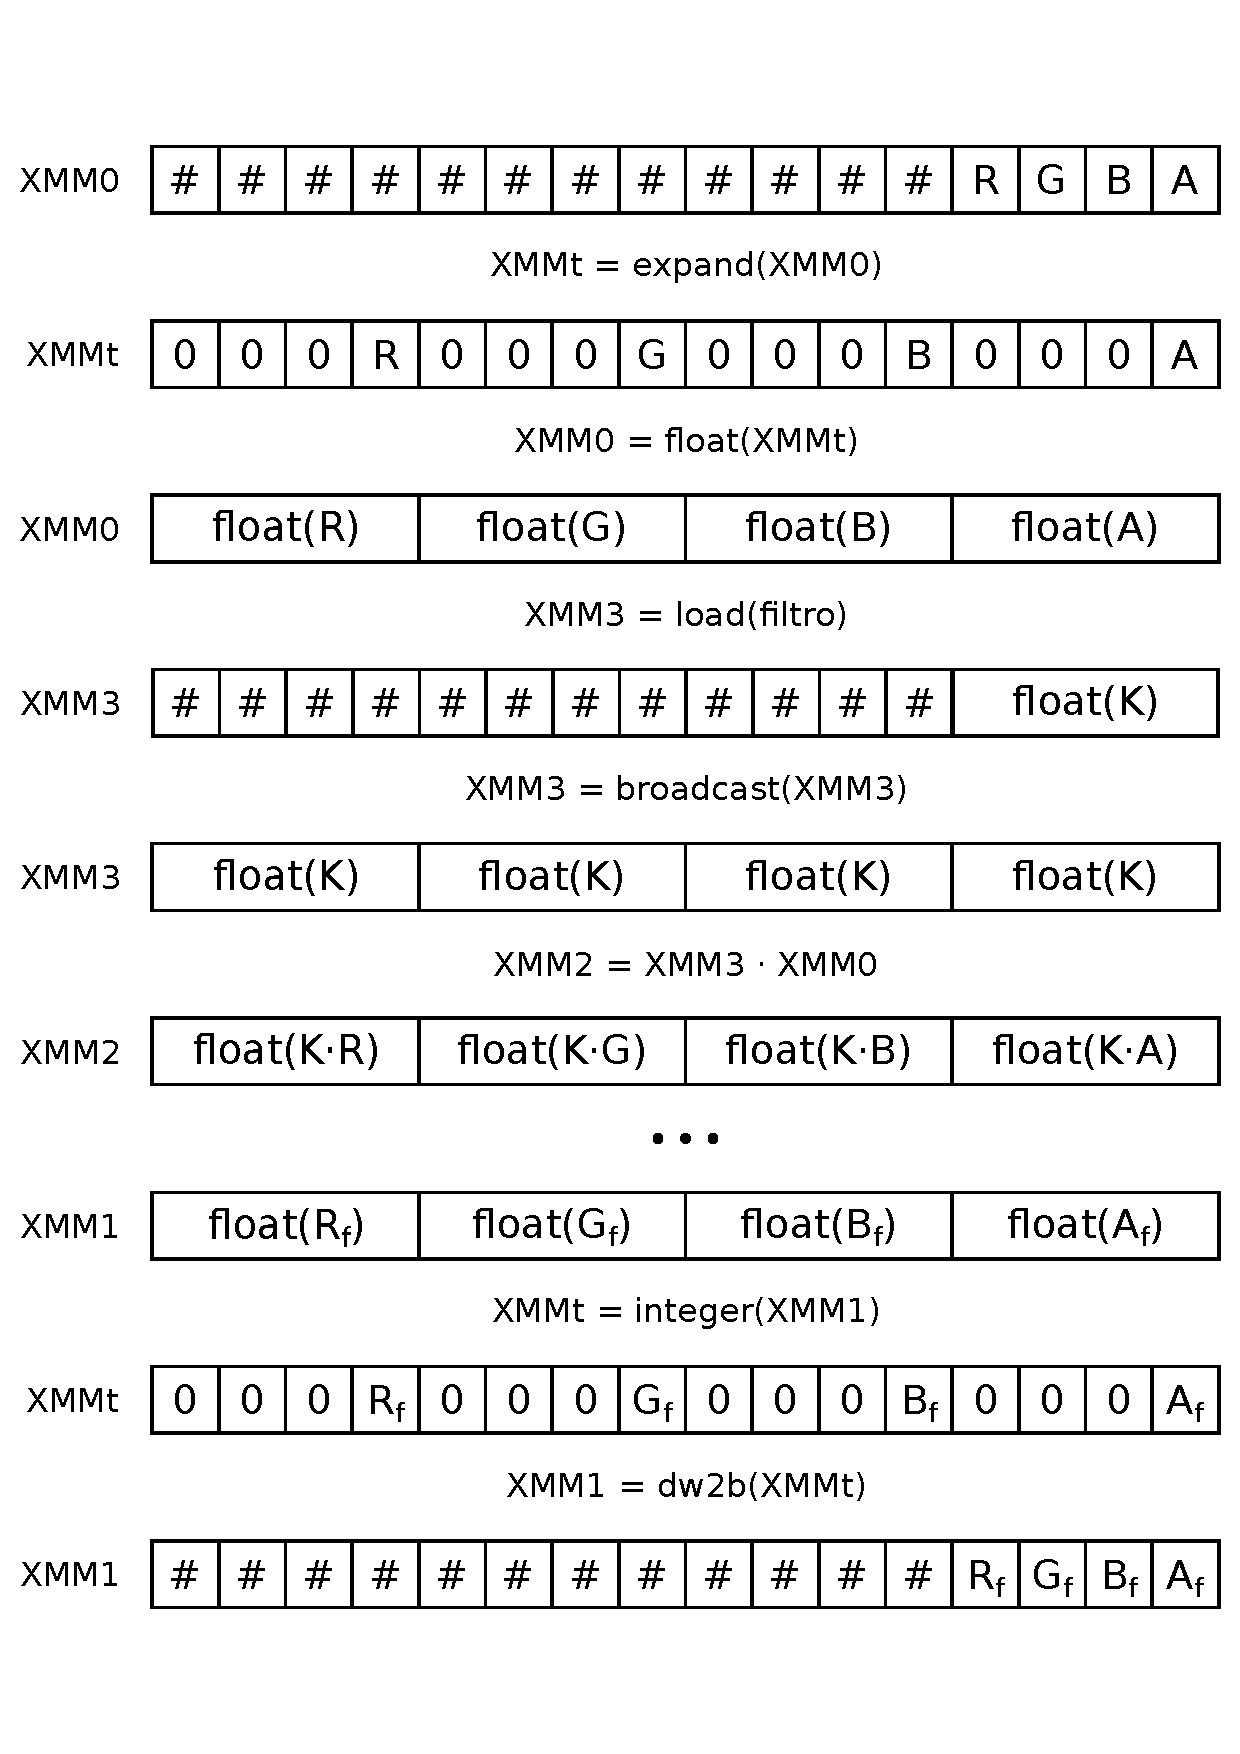
\includegraphics[width=0.7\columnwidth]{esquema_blur.pdf}
  \caption{Esquema que caracteriza el algoritmo de blur con
    instrucciones {\ttfamily SIMD}}
  \label{fig:esquema_blur}
\end{figure}


Terminado esto, ¡ya tenemos procesado el píxel! Hacemos esto para toda
la fila [sumando de a 4 bytes para pasar al siguiente elemento] y,
para evitar el \emph{marco}, en el último elemento de la fila sumamos
$2\,r \, 4\text{bytes}$ para pasar al siguiente elemento del
\emph{centro}.

